\documentclass[a4paper,12pt]{article}
\usepackage[utf8]{inputenc}
\usepackage{fontspec} 
%\XeTeXlinebreaklocale "zh" 
%\XeTeXlinebreakskip = 0pt plus 1pt 
%\setmainfont[Mapping=tex-text]{DejaVu Serif} % rm
\usepackage{graphicx}
\usepackage[a4paper]{geometry}
%\setlength{\textwidth}{5in}
%\setlength{\hoffset}{0.6in}
%header
\usepackage{fancyhdr}
%math package
\usepackage[fleqn]{amsmath}
%\usepackage{amsmath,amssymb}
%code package
%\usepackage{minted}
\usepackage{listings}
\usepackage{minted}
\usepackage[lined,boxed]{algorithm2e}
\usepackage{subcaption}

\newcommand{\horrule}[1]{\rule{\linewidth}{#1}} 
\title{	
\normalfont \normalsize \vspace{-13em} % Your university, school and/or department name(s)
\horrule{1pt} \\[0.5cm] % Thick bottom horizontal rule
\huge Neural Network
\\ % The assignment title
\vspace{1em}
\large Assignment 4
\horrule{2pt} \\[0.5cm] % Thick bottom horizontal rule
}
\author{Zhao Shenjian 5110309748}
\date{}
\pagestyle{fancy}
\rhead{Self Organizing Map}


\begin{document}   
\maketitle
\thispagestyle{empty}
\setcounter{page}{1}
\section*{Part I: Self-organizing maps}
  \paragraph{}A self-organizing map is a type of artificial neural network (ANN) that is trained using unsupervised learning to produce a low-dimensional,
  discretized representation of the input space of the training samples, called a map. 
  Self-organizing maps are different from other artificial neural networks in the sense that they use a neighborhood function to preserve the 
  topological properties of the input space.
  \paragraph{} In this homework, we are mapping two gaussian distributions to $ 5*5 $ neural network.
  
 \section*{Part II: Matlab implementation}
 \paragraph{} According to the algorithm, we can easily implement it in Matlab. But there are some parameters to tweak such as the learning rate and the 
 gaussian neighborhood function.

 \section*{Part III: Test results}
\paragraph{} I run this implementation with different parameters, and the results is shown in the following figures.
With larger learning rate the results will converge slower, but smaller learning rate and $\sigma$ will produce
incorrect results.

 
 
\begin{figure}[h!]
\begin{center}
%\framebox[4.0in]{$\;$}

\begin{subfigure}{.33\textwidth}
  \centering
  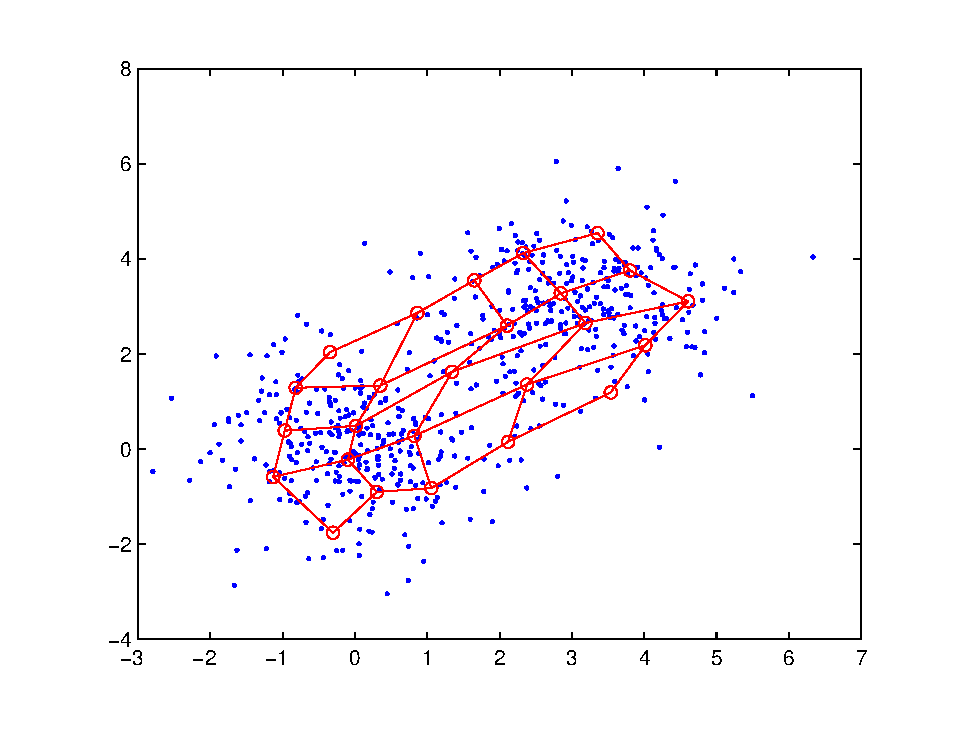
\includegraphics[width=.8\linewidth]{p1000}
      \caption{learning rate 1000, $ \sigma = 4 $}
\end{subfigure}%
\begin{subfigure}{.33\textwidth}
  \centering
  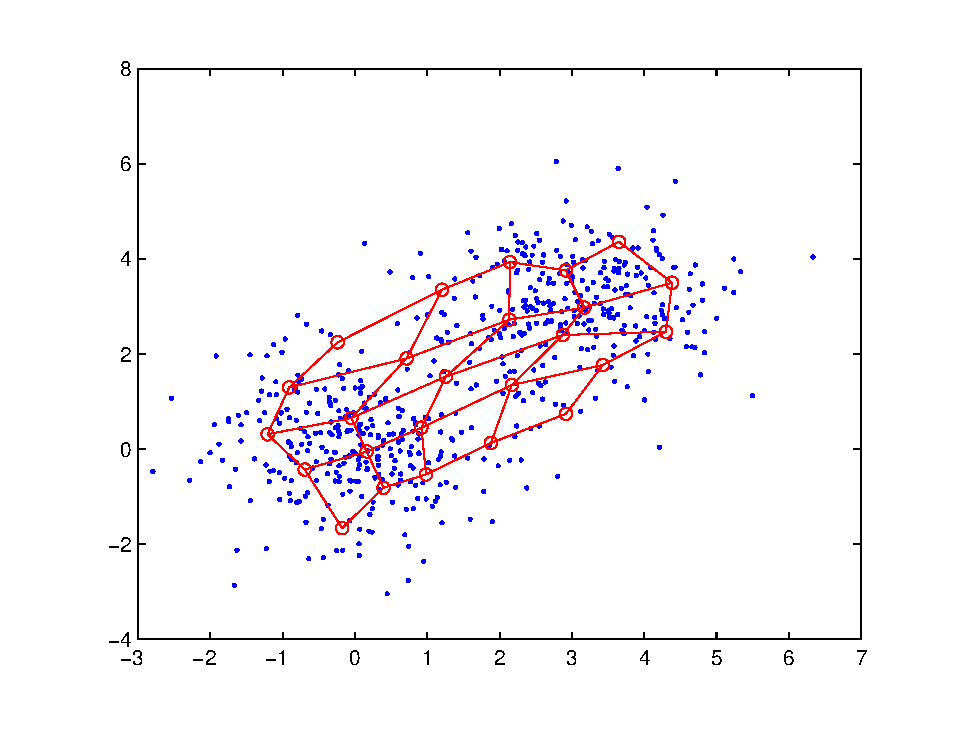
\includegraphics[width=.8\linewidth]{p500}
      \caption{learning rate 500, $ \sigma = 4 $}
\end{subfigure}%
\begin{subfigure}{.33\textwidth}
  \centering
  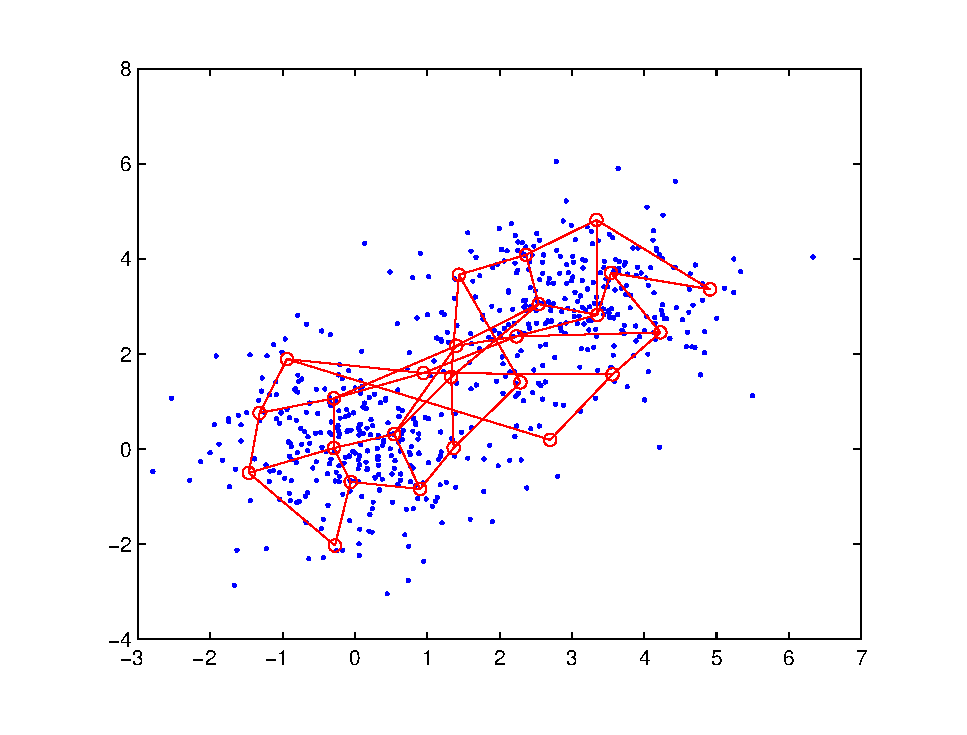
\includegraphics[width=.8\linewidth]{rho1}
      \caption{learning rate 500, $ \sigma = 1 $}
\end{subfigure}%
\end{center}
      \caption{Comparison of different parameters}
      \end{figure}
      
      
 

\end{document} 
